\documentclass[color=blue, thmcnt=section, 12pt]{elegantbook}

% Title and author
\title{Machine Learning}
\author{Isaac FEI}

\cover{cover}

\begin{document}

% Print title and cover page
\maketitle

% Print table of contents
\frontmatter
\tableofcontents
\mainmatter

%------------------------------
% Main document starts from here
%------------------------------



%==============================
%==============================

\part{Elementary Concepts}

%==============================
%==============================






%------------------------------

\chapter{Singular Value Decomposition (SVD)}

%------------------------------

\section{A Geometric Interpretation}

\begin{theorem}
    Let $A$ be an $m \times n$ real matrix with rank $r$. Then $A$ can be decomposed by 
    \begin{align*}
        A = U \Sigma V^\top
    \end{align*}
    where $U$ and $V$ are orthogonal matrices with shape $m \times m$ and $n \times n$, respectively. $\Sigma$ is an $m \times n$ matrix in the form of
    \begin{align*}
        \left[ \begin{array}{ccc|c}
            \sigma_1 &  & & \\ 
            & \ddots & & 0 \\ 
            & & \sigma_r & \\ 
            \hline
            & 0 & & 0
        \end{array} \right]
    \end{align*}
    where $\sigma_1, \ldots, \sigma_r$ are nonnegative numbers satisfying
    \begin{align*}
        \sigma_1 \geq \cdots \geq \sigma_r > 0
    \end{align*}
\end{theorem}

\begin{proof}
    % TODO
\end{proof}

%------------------------------

\section{Image Compression}

\par Given a color image with height $m$ (pixels) and width $n$ (pixels), we first split the RGB channels. Then, each channel is regarded as an $m \times n$ matrix $A$. Applying the SVD to $A$, we obtain
\begin{align*}
    A = U \Sigma V^\top
\end{align*}
In practice, $A$ is very likely to have full rank, which means it has as many singular values as possible (at most $\min\left\{m, n\right\}$ singular values). But not all singular values along with its associated left and right singular vectors are of the same importance to the image, which we will explain in the following way.

\par For a pixel $a_{ij}$ located at the $i$-th row and $j$-th column in the image $A$, its value equals to 
\begin{align*}
    a_{ij} = \sum_{k=1}^n \sigma_k u_{ik} v_{jk}
\end{align*}
If the singular value $\sigma_k$ becomes very small starting from $k \geq r+1$, then the sum $\sum_{k=r+1}^n \sigma_k u_{ik} v_{jk}$ has little contribution to the pixel value $a_{ij}$. Hence, $a_{ij}$ can be approximated by 
\begin{align*}
    a_{ij} \approx \sum_{k=1}^r \sigma_k u_{ik} v_{jk}
\end{align*}

\par In this way, the original image $A$ can be compressed by only keeping the first $r$ singular values while dropping the rest. Mathematically, the compressed image $\hat{A}$ is given by
\begin{align*}
    \hat{A} = \hat{U} \hat{\Sigma} \hat{V}^\top
    = \begin{bmatrix}
        \mathbf{u}_1 & \cdots & \mathbf{u}_r
    \end{bmatrix} \begin{bmatrix}
        \sigma_1 & & \\ 
        & \ddots & \\ 
        & & \sigma_r
    \end{bmatrix} \begin{bmatrix}
        \mathbf{v}^\top_1 \\ \vdots \\ \mathbf{v}^\top_r
    \end{bmatrix}
\end{align*}
Recall $A$ represents a single channel. The final compressed color image can be then generated by merging all three compressed images from each channel.

\par We now demonstrate the algorithm to compress the image shown in Figure~\ref{fig:1} in Python.
\begin{figure}[h!]
    \centering
    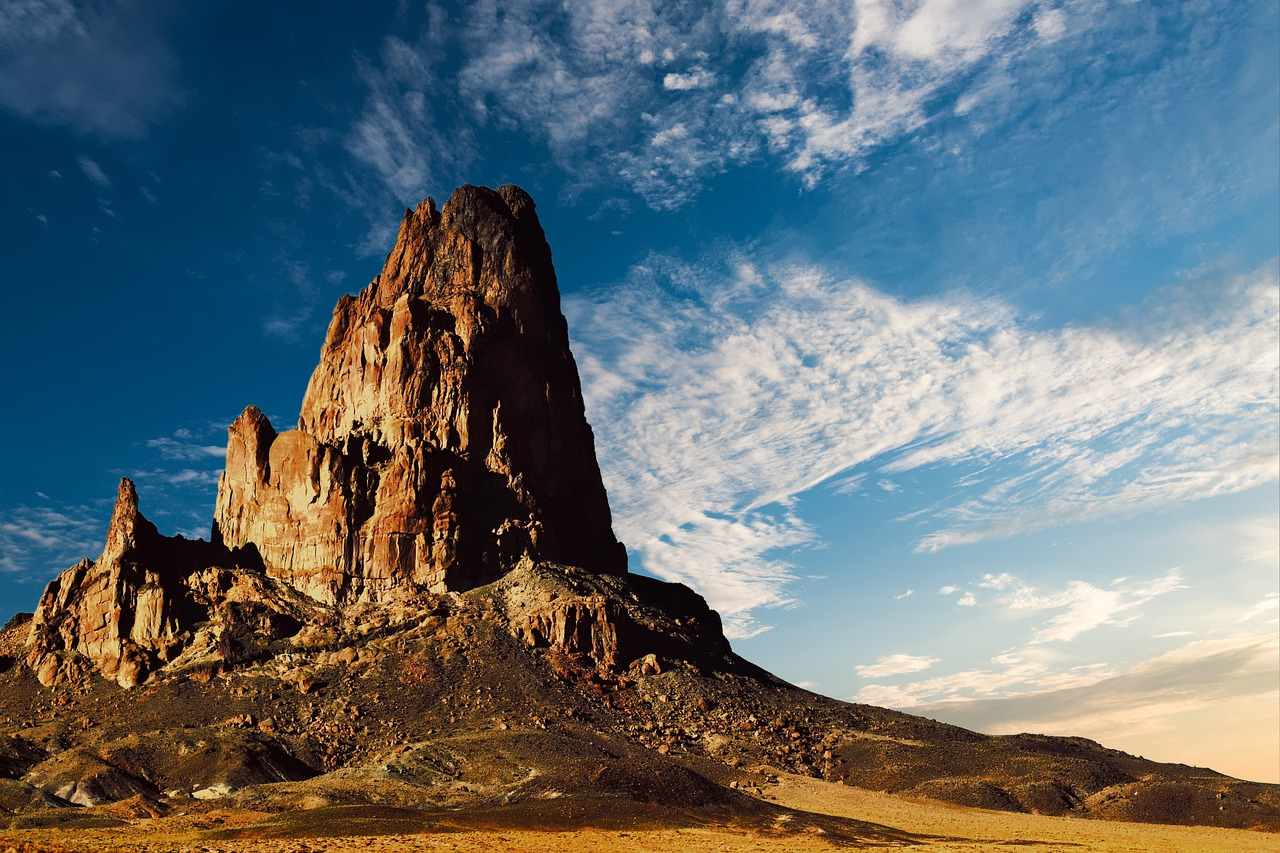
\includegraphics[scale=0.1]{figures/mountain.jpg}
    \caption{Mountain}
    \label{fig:1}
\end{figure}

\par The Python code is listed below. The parameter \texttt{r} in function \verb|compress_image| is the number of singular values we want to keep after compression.
\begin{lstlisting}[language=Python]
# open image file
img: Image.Image = Image.open("./data/mountain.jpg")

def compress_channel(A: np.ndarray, r: int) -> np.ndarray:
    # SVD
    U, s, Vh = svd(A)
    
    # keep first r singular values
    U = U[:, :r]
    s = s[:r]
    Vh = Vh[:r, :]
    A_hat = (U * s) @ Vh 
    
    # clip pixel values
    A_hat = np.clip(A_hat, a_min = 0, a_max = 255)
    A_hat = A_hat.astype(np.uint8)
    
    return A_hat

def compress_image(img: Image.Image, r: int) -> Image.Image:
    # split RGB channels
    channels: list[Image.Image] = img.split()
    
    compressed_channels = []
    for channel in channels:
        # convert image to NumPy array
        A = np.array(channel)
        
        # compress single channel
        A_hat = compress_channel(A, r)
        
        # convert to Image class instance
        channel = Image.fromarray(A_hat)
        compressed_channels.append(channel)
    
    # merge channels
    compressed_img = Image.merge("RGB", compressed_channels)
    
    return compressed_img
\end{lstlisting}

\begin{note}
    It is important to clip the pixel values as in line 15. If this line is omitted, then the resulting compressed image is not as expected.
\end{note}

\par Figure~\ref{fig:2} shows the result of the compressed images with \texttt{r = 10} and \texttt{r = 50}. The size of the original image is 380 KB. After compression, the size reduces to 97 KB and 154 KB, respectively.

\begin{figure}[h!]
    \centering
    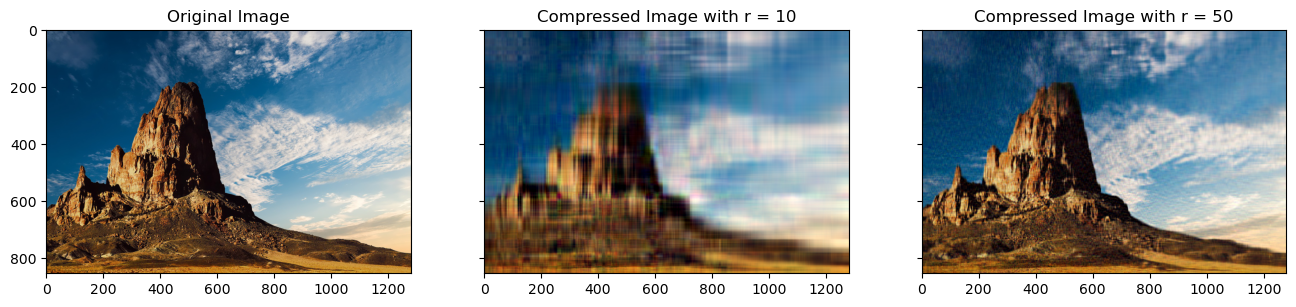
\includegraphics[scale=0.5]{figures/compressed-images.png}
    \caption{Original Image and Its Compressed Images}
    \label{fig:2}
\end{figure}

\par When \texttt{r} is 10, the compressed image is rather vague. But when \texttt{r} rises to 50, the decline in image quality is seamless.

\begin{proposition}
    Suppose $A \in \FF^{m \times n}$, $B \in \FF^{n \times k}$ and $C \in \FF^{l \times n}$ where $\FF$ is either $\R$ or $\C$. Then we have the following properties:
    \begin{enumerate}
        \item If $\rank(B) = n$, then $\rank(AB) = \rank(A)$.
        \item If $\rank(C) = m$, then $\rank(CA) = \rank(A)$.
    \end{enumerate}
\end{proposition}

\begin{remark}
    One may suggest replacing the condition $\rank(B) = n$ with that $B$ has full rank in statement 1. But in general, that is not true. For example, suppose $A$ is a $2 \times 2$ invertible matrix and $B$ is a non-zero column vector. Then it is clear that $A$ has rank $2$ and $B$ has full rank (rank $1$). But $AB$ is a column vector, which has rank $1$ instead of $2$. Similarly, we cannot replace the condition $\rank(C) = m$ with that $C$ has full rank in statement 2.
\end{remark}

%------------------------------

\section{Optimal Hard Threshold for Singular Values}



%------------------------------

\section{Face Recognition}

%------------------------------

\section{Edge Detection: An Example of Complex-Valued Datasets}

%------------------------------

%==============================

\chapter{Dimensionality Reduction}

%==============================

\section{Curse of Dimensionality}

%------------------------------

\section{Principal Component Analysis (PCA)}

%------------------------------

\begin{definition}
    Let $\mathbf{X} = \left[X_1 \cdots X_n\right]^\top$ be an $n$-dimentional vector of random variables. Suppose $\mathbf{v}_1, \ldots, \mathbf{v}_n$ are $n$ unit vectors. Define random variable
    \begin{align*}
        T_j = \mathbf{v}_j^\top \mathbf{X}
        \quad 1 \leq j \leq n
    \end{align*}
    Then we say $\mathbf{v}_j$ is the $j$-th \textbf{principal component} \index{principal component} of $\mathbf{X}$ if $\mathbf{v}_j$ is the solution to the following optimization problem:
    \begin{alignat}{2}
        \max_{\mathbf{v}_j}&\quad & &\var(T_j) \label{eq:1}\\ 
        \text{s.t.}& & &\begin{cases}
            \mathbf{v}_j^\top \mathbf{v}_j = 1 \nonumber\\
            \cov(T_i, T_j) = 0 \quad \forall 1 \leq i \leq j-1
        \end{cases}
    \end{alignat}
    In this case, $T_j$ is called the \textbf{principal component score} \index{principal component score} for $\mathbf{v}_j$.
\end{definition}

\begin{remark}
    Note that the principal component scores $T_1, \ldots, T_n$ are mutually uncorrelated, i.e., 
    \begin{align*}
        i \neq j \implies \cov(T_i, T_j) = 0 
    \end{align*}
\end{remark}

%------------------------------

\par Now, we have formulated the rigorous definition of the principal components, which captures the idea of preserving the maximum variance of the data. But what are the principal components exactly, and how can we find them? As stated in the above definition, the principal component $\mathbf{v}_j$ can be found by solving the optimization problem \eqref{eq:1}.

\par The following theorem provides the solution to \eqref{eq:1}. To our surprise, the $j$-th principal component is the $j$-th eigenvector of the covariance matrix $\cov(\mathbf{X}, \mathbf{X})$ if the eigenvalues are sorted in the decreasing order.

%------------------------------

\begin{theorem}
    Suppose that $\mathbf{X} = \left[X_1 \cdots X_n\right]^\top$ is an $n$-dimentional vector of random variables. Let $\Sigma = \cov(\mathbf{X}, \mathbf{X})$ denote the covariance matrix. Since $\Sigma$ is positive semi-definite, it has $n$ nonnegative eigenvalues, say $\lambda_1, \ldots, \lambda_n$. We may assume that these eigenvalues are sorted in the descending order, i.e., 
    \begin{align*}
        \lambda_1 \geq \cdots \geq \lambda_n \geq 0
    \end{align*}
    Let $\mathbf{v}_1, \ldots, \mathbf{v}_n$ be the corresponding orthonormal eigenvectors. Then $\mathbf{v}_j$ is precisely the $j$-th principal component of $\mathbf{X}$.
\end{theorem}

\par The general idea of this proof is to solve \eqref{eq:1} with the method of Lagrange multiplier.

\begin{proof}
    (Covariance as Matrix multiplications) We first write $\cov(T_i, T_j)$ in the form of matrix multiplications. We have 
    \begin{align*}
        \cov(T_i, T_j)
        &= \cov\left(
            \mathbf{v}_i^\top \mathbf{X},
            \mathbf{v}_j^\top \mathbf{X}
        \right) \\ 
        &= \cov\left(
            \sum_{k=1}^n v_{ik} X_k,
            \sum_{l=1}^n v_{jl} X_l
        \right) \\ 
        &= \sum_{k=1}^n \sum_{l=1}^n v_{ik} v_{jl} \cov(X_k, X_l) \\ 
        &= \mathbf{v}_i^\top \Sigma \mathbf{v}_j
    \end{align*}
    In summary, 
    \begin{align*}
        \cov(T_i, T_j) = \mathbf{v}_i^\top \Sigma \mathbf{v}_j
    \end{align*}
    Specially, when $i = j$ we have
    \begin{align*}
        \var(T_j) = \mathbf{v}_j^\top \Sigma \mathbf{v}_j
    \end{align*}

    \par (Induction Hypothesis) We shall prove this theorem by induction. The induction hypothesis is stated as follows.
    \begin{align}
        P(m): \mathbf{v}_1, \ldots, \mathbf{v}_m \text{ are the first $m$ principal components.}
        \label{eq:7}
    \end{align}

    \par (Base Case: The First Principal Component) Consider the optimization problem \eqref{eq:1} for $j = 1$:
    \begin{alignat}{2}
        \max_{\mathbf{v}}&\quad & &\var(T) = \var(\mathbf{v}^\top \mathbf{X}) = \mathbf{v}^\top \Sigma \mathbf{v} \label{eq:2}\\ 
        \text{s.t.}& & &\mathbf{v}^\top \mathbf{v} = 1 \nonumber
    \end{alignat}
    Note that in this case, there is only one constraint $\mathbf{v}^\top \mathbf{v} = 1$. The Lagrangian function is given by 
    \begin{align*}
        \mathcal{L}(\mathbf{v}; \lambda)
        = \mathbf{v}_1^\top \Sigma \mathbf{v} - \lambda \mathbf{v}^\top \mathbf{v}
    \end{align*}
    Taking the partial derivative with respect to $\mathbf{v}$, we obtain
    \begin{align*}
        \frac{\partial \mathcal{L}}{\partial \mathbf{v}} = 2 \Sigma \mathbf{v} - 2\lambda \mathbf{v}
    \end{align*}
    Letting the partial derivative equal to zero, it follows that 
    \begin{align*}
        (\Sigma - \lambda I)\mathbf{v} = \mathbf{0}
    \end{align*}
    This implies $\lambda$ is an eigenvalue of $\Sigma$ and $\mathbf{v}$ is its corresponding eigenvector. Then, the variance we want to maximize in \eqref{eq:2} reduces to 
    \begin{align*}
        \var(T)
        = \mathbf{v}^\top \Sigma \mathbf{v}
        = \lambda \mathbf{v}^\top \mathbf{v}
        = \lambda
    \end{align*}
    Therefore, the maximum of $\var(T) = \lambda$ is $\lambda_1$. And then the optimal solution $\mathbf{v}_1$ is the eigenvector corresponding to $\lambda_1$.

    \par (Inductive Step) Assume the induction hypothesis \eqref{eq:7} holds for $k$, i.e., $P(k)$ holds. Now, consider the optimization problem:
    \begin{alignat}{2}
        \max_{\mathbf{v}}&\quad & &\var(T) = \var(\mathbf{v}^\top \mathbf{X}) = \mathbf{v}^\top \Sigma \mathbf{v} \label{eq:3}\\ 
        \text{s.t.}& & &\begin{cases}
            \mathbf{v}^\top \mathbf{v} = 1 \nonumber\\
            \cov(T_i, T) = 0 \quad \forall 1 \leq i \leq k
        \end{cases}
    \end{alignat}
    Recall we have shown $\cov(T_i, T) = \mathbf{v}_i^\top \Sigma \mathbf{v} = \mathbf{v}^\top \Sigma \mathbf{v}_i$. And since $\mathbf{v}_i$ is an eigenvector corresponding to $\lambda_i$, it follows that
    \begin{align*}
        \cov(T_i, T) 
        = \mathbf{v}^\top \Sigma \mathbf{v}_i 
        = \lambda_i \mathbf{v}^\top \mathbf{v}_i
        = \lambda_i \mathbf{v}_i^\top \mathbf{v}
    \end{align*}
    Therefore, the problem \eqref{eq:3} is reduced to 
    \begin{alignat}{2}
        \max_{\mathbf{v}}&\quad & &\var(T) = \var(\mathbf{v}^\top \mathbf{X}) = \mathbf{v}^\top \Sigma \mathbf{v} \label{eq:4}\\ 
        \text{s.t.}& & &\begin{cases}
            \mathbf{v}^\top \mathbf{v} = 1 \nonumber\\
            \lambda_i \mathbf{v}_i^\top \mathbf{v} = 0 \quad \forall 1 \leq i \leq k
        \end{cases}
    \end{alignat}
    The Lagrangian function is then given by 
    \begin{align*}
        \mathcal{L}(\mathbf{v}; \lambda, \phi_1, \ldots, \phi_k)
        = \mathbf{v}^\top \Sigma \mathbf{v}
        - \lambda(\mathbf{v}^\top \mathbf{v} - 1)
        - \phi_1 \lambda_1 \mathbf{v}_1^\top \mathbf{v}
        - \cdots 
        - \phi_k \lambda_k \mathbf{v}_k^\top \mathbf{v}
    \end{align*}
    The partial derivative of $\mathbf{v}$ is 
    \begin{align*}
        \frac{\partial \mathcal{L}}{\partial \mathbf{v}}
        = 2 \Sigma \mathbf{v} - 2\lambda \mathbf{v}
        - \phi_1 \lambda_1 \mathbf{v}_1
        - \cdots
        - \phi_k \lambda_k \mathbf{v}_k
    \end{align*}
    
    \par $\frac{\partial \mathcal{L}}{\partial \mathbf{v}} = \mathbf{0}$ yields that 
    \begin{align}
        (\Sigma - \lambda I) \mathbf{v}
        = \frac{1}{2} (
            \phi_1 \lambda_1 \mathbf{v}_1
            + \cdots
            + \phi_k \lambda_k \mathbf{v}_k
        )
        \label{eq:5}
    \end{align}
    For each vector $\mathbf{v}_j$ ($1 \leq j \leq k$), we have 
    \begin{align*}
        \mathbf{v}_i^\top \mathbf{v} = 0
    \end{align*}
    due to the constraint of \eqref{eq:4}. Moreover, 
    \begin{align*}
        \mathbf{v}_i^\top \mathbf{v}_j = \begin{cases}
            1 &i = j \\ 
            0 &i \neq j
        \end{cases}
    \end{align*}
    due to the hypothesis. Then Taking the inner product with $\mathbf{v}_i$ on both sides of \eqref{eq:5}, we obtain
    \begin{align}
        0 = (\Sigma - \lambda I) \mathbf{v}_i^\top \mathbf{v}
        = \frac{1}{2} (
            \phi_1 \lambda_1 \mathbf{v}_i^\top\mathbf{v}_1
            + \cdots
            + \phi_k \lambda_k \mathbf{v}_i^\top\mathbf{v}_k
        )
        = \frac{1}{2} \phi_i \lambda_i
        \quad \forall 1 \leq i \leq k
        \label{eq:6}
    \end{align}
    Equation \eqref{eq:6} yields that
    \begin{align*}
        \phi_i \lambda_i = 0 
        \quad \forall 1 \leq i \leq k
    \end{align*}
    Then \eqref{eq:5} reduces to 
    \begin{align*}
        (\Sigma - \lambda I) \mathbf{v} = \mathbf{0}
    \end{align*}
    This implies $\lambda$ is an eigenvalue of $\Sigma$ and $\mathbf{v}$ is its corresponding eigenvector. Recall problem \eqref{eq:4}. We want to maximize 
    \begin{align*}
        \var(T) = \mathbf{v}^\top \Sigma \mathbf{v}
        = \lambda \mathbf{v}^\top \mathbf{v}
        = \lambda
    \end{align*}
    
    \par Hence, we want $\lambda$ to be as large as possible. And the optimal choice is $\lambda = \lambda_{k+1}$ because $\lambda$ cannot be $\lambda_i$ ($1 \leq i \leq k$) if $\lambda_i > \lambda_{k+1}$. Otherwise, $\lambda = \lambda_i$ would imply that $\mathbf{v}$ being an eigenvector of $\lambda_i$, which would lead to a contradiction since all the independent eigenvectors are already included among $\mathbf{v}_1, \ldots, \mathbf{v}_k$. In conclusion, the solution to problem \eqref{eq:4} is $\mathbf{v} = \mathbf{v}_{k+1}$.

    \par This completes the proof.
\end{proof}

%------------------------------



%------------------------------

\end{document}